%% Supplementary Material for "Overlapping construction plus a position-blind split".
%% Standalone document. Sections numbered S1, S2, ...; figures and tables S1, S2, ...
%% Companion to paper/main_resubmission.tex. Numbers here trace to the same results/*.csv files.
%% tab_roster.tex is GENERATED by audit.pipeline.emit_tables -- never edit it by hand.
\documentclass[11pt,a4paper]{article}

\usepackage[margin=2.4cm]{geometry}
\usepackage{amsmath}
\usepackage{booktabs}
\usepackage{graphicx}
\usepackage{multirow}
\usepackage{natbib}
\usepackage{url}
\usepackage[colorlinks=true,allcolors=blue]{hyperref}

\graphicspath{{Fig/}}
\emergencystretch=3em
\sloppy
\bibliographystyle{oup-abbrvnat}

\renewcommand{\thesection}{S\arabic{section}}
\renewcommand{\thesubsection}{S\arabic{section}.\arabic{subsection}}
\renewcommand{\thetable}{S\arabic{table}}
\renewcommand{\thefigure}{S\arabic{figure}}
\renewcommand{\theequation}{S\arabic{equation}}
\providecommand{\botrule}{\bottomrule}

\title{Supplementary Material\\[3pt]
\large Overlapping construction plus a position-blind split:\\
a curation defect in genomic sequence benchmarks and the model rankings it inverts}
\author{Rikhin Kavuru}
\date{}

\begin{document}
\maketitle

\noindent Section numbers of the form \S3.6 refer to the main text; \S S1, \S S2, \dots\ refer to
this document. Every number here is re-derived from the CSV files released with the code, and the
gate script \texttt{audit/tools/check\_numbers.py} checks both documents against those files.

\tableofcontents

\section{Extended methods}\label{sec:s-methods}

\subsection{Datasets}\label{sec:s-data}

\begin{table}[htbp]
\centering
\caption{Datasets in the Genomic Benchmarks binary suite, and the optional three-class set.
Lengths are the median with min--max range where variable; class balance is the positive-class
fraction. All balanced datasets are curated to $0.500$ in both train and test, so balance is
preprocessed rather than natural.}\label{tab:datasets}
\footnotesize\setlength{\tabcolsep}{6pt}
\begin{tabular}{@{}lrlll@{}}
\toprule
Dataset & $n$ (full) & Length (bp) & Class balance & Test fraction\\
\midrule
human\_nontata\_promoters            & 36{,}131  & 251              & 0.544 & 0.25\\
human\_enhancers\_ensembl            & 154{,}842 & 269 (2--573)     & 0.500 & 0.20\\
human\_ocr\_ensembl                  & 174{,}756 & 315 (71--593)    & 0.500 & 0.20\\
human\_enhancers\_cohn               & 27{,}791  & 500              & 0.500 & 0.25\\
demo\_coding\_vs\_intergenomic\_seqs & 100{,}000 & 200              & 0.500 & 0.25\\
demo\_human\_or\_worm                & 100{,}000 & 200              & 0.500 & 0.25\\
drosophila\_enhancers\_stark         & 6{,}914   & 2142 (236--3237) & 0.500 & 0.25\\
\midrule
human\_ensembl\_regulatory (3-class) & 289{,}061 & 401 (89--802)    & 3 classes & 0.20\\
\bottomrule
\end{tabular}
\end{table}

\subsection{Model roster: full specification}\label{sec:s-roster}
The four-model comparison used for the report card is: logistic regression (\texttt{C=1.0},
\texttt{max\_iter=5000}); a linear support-vector machine (\texttt{LinearSVC}, \texttt{C=1.0},
\texttt{dual=False}, \texttt{max\_iter=5000}); a random forest (\texttt{n\_estimators=150},
scikit-learn defaults \texttt{min\_samples\_leaf=1}, \texttt{max\_depth=None}); and gradient-boosted
trees (\texttt{HistGradientBoosting}, library defaults). The nine-model roster reuses those four
\emph{verbatim}---same objects, same normalization, same seeds---and adds: $1$- and $15$-nearest
neighbours; extremely randomized trees (\texttt{n\_estimators=150}, defaults); a multilayer
perceptron (one hidden layer of $128$ units, \texttt{early\_stopping=True}, \texttt{max\_iter=60});
and Gaussian naive Bayes. The model seed is $0$ throughout.

The roster spans memorization propensity end to end rather than accuracy. $1$-nearest-neighbour is
the definitional memorizer---on a near-duplicate its prediction simply \emph{is} the training
label---so it bounds the axis from above; Gaussian naive Bayes bounds it from below.
$15$-nearest-neighbour was designated memorization-prone in advance and turns out to sit at the
bottom of the corrected-gap ordering, because averaging over fifteen neighbours is what stops a
nearest-neighbour rule from memorizing; we keep it in the memorization-prone set as registered
rather than reclassifying it after the fact.

\paragraph{Normalization policy.} L2 normalization is applied via a \texttt{Normalizer} pipeline
step to the scale-sensitive learners only: both linear models, both nearest-neighbour rules and the
MLP. The tree ensembles consume raw $k$-mer counts, for which monotone feature scaling is
irrelevant, and Gaussian naive Bayes standardizes internally.

\paragraph{Feature settings.} Overlapping $k$-mer counts at $k\in\{4,6\}$; main-text results use
$k=6$ unless stated. At $k=4$ the demotion reproduces, with full-scale random-forest drops of
$0.153$ and $0.084$ on the two leaky datasets and the demotion holding under accuracy and AUROC
alike. The three-class row of the report card is a $k=4$ figure.

The nine-model roster itself is Table~3 of the main text, which carries, per model, both forms of
the graded memorization gap, the as-shipped and corrected accuracies, the drop with its two-arm
cluster-bootstrap interval, and the rank on each split.

\paragraph{Reading conventions for the roster.} An inversion criterion designed for four models is
too permissive for nine, because with a wider roster the top two are often within noise and a
``top model changed by more than a point'' rule fires on a \emph{clean} control from repartitioning
alone; hence the two-arm paired requirement stated in the main text. And the margin between the two
models that \emph{swap} is a different quantity from the margin between as-shipped first and second
place: the latter can be a statistical tie while the former is large, which is the situation on
\textit{human\_enhancers\_ensembl}.

\subsection{The prevalence-corrected graded memorization gap}\label{sec:s-gap}
The split-internal graded memorization gap is
\begin{equation}
g_M \;=\; \mathrm{acc}_M[\,s\ge0.9\,]\;-\;\mathrm{acc}_M[\,s<0.5\,],
\end{equation}
for $s$ the maximum $8$-mer Jaccard of a test sequence to any training sequence. Raw, the statistic
is confounded by stratum class composition. The $\ge0.9$ stratum is $99.97\%$ positive on
\textit{human\_enhancers\_ensembl} against $19.68\%$ in the novel stratum, and $0.15\%$ against
$98.17\%$ on \textit{human\_nontata\_promoters}---opposite directions on the two datasets. A
constant classifier that always predicts the positive class, and therefore memorizes nothing,
scores a raw gap of $+0.803$ on the first and $-0.980$ on the second, so any model with a
class-prediction bias inherits a large gap of the corresponding sign for free.

We therefore compute the gap from \emph{balanced} accuracy---the unweighted mean of per-class
recall---within each stratum. A constant classifier scores $0.5$ in every stratum under that
definition, hence a corrected gap of exactly zero. Both forms appear side by side in
Table~\ref{tab:roster} so the size of the confound is visible. The correction disposes of two raw
values never interpretable as memorization: $15$-nearest-neighbour's raw $-0.684$ and naive Bayes's
$-0.234$ become $+0.016$ and $+0.129$, i.e.\ artifacts of predicting the minority class in a
stratum that is $99.97\%$ positive.

\begin{table}[htbp]
\centering
\caption{Nine-model roster on \textit{human\_enhancers\_ensembl}, full scale, as-shipped versus
near-duplicate-aware split. Gap$_{\text{bal}}$ is the graded memorization gap computed from
\emph{balanced} accuracy within each stratum and is the statistic relied on; Gap$_{\text{raw}}$ is
the uncorrected accuracy difference, shown only for comparison because it is confounded by stratum
class composition---a constant classifier scores $+0.803$ on this dataset, which is why the raw
column carries two large negative values that do not indicate ``negative memorization''. The
corrected column orders the models as the memorization account predicts and the raw column does
not. ``Drop'' is the accuracy lost under correction, with a two-arm cluster-bootstrap interval;
$^{*}$ marks intervals excluding zero. Models are ordered by as-shipped rank. The top three
as-shipped finish within $0.0015$ of one another---a tie---yet span $23$ points on the corrected
split, and the corrected winner is the linear SVM. Generated from
\texttt{results/roster\_rankings.csv}; the prevalence-corrected gaps are exploratory
(main text \S3.7).\label{tab:roster}}
\footnotesize\setlength{\tabcolsep}{3pt}% GENERATED by audit/pipeline/emit_tables.py -- do not edit by hand.
% Edit the source CSV and re-run, or the next build will overwrite you.
\begin{tabular}{@{}lrrrrrl@{}}
\toprule
Model & Gap$_{\text{bal}}$ & Gap$_{\text{raw}}$ & As-shipped & Corrected & Drop & Rank\\
\midrule
MLP & \textbf{0.234} & $0.159$ & \textbf{0.8736} & 0.7684 & $0.105^{*}$ & $1\!\to\!3$\\
kNN-1 & \textbf{0.461} & $0.208$ & 0.8729 & 0.5370 & $0.336^{*}$ & $2\!\to\!9$\\
ExtraTrees & \textbf{0.370} & $0.210$ & 0.8721 & 0.6278 & $0.244^{*}$ & $3\!\to\!7$\\
RandomForest & \textbf{0.319} & $0.230$ & 0.8596 & 0.6957 & $0.164^{*}$ & $4\!\to\!5$\\
LinearSVC & \textbf{0.144} & $0.037$ & 0.7980 & \textbf{0.7975} & $0.001$ & $5\!\to\!1$\\
LogisticReg. & \textbf{0.154} & $0.037$ & 0.7809 & 0.7806 & $0.000$ & $6\!\to\!2$\\
HistGB & \textbf{0.162} & $0.034$ & 0.7636 & 0.7608 & $0.003$ & $7\!\to\!4$\\
GaussianNB & \textbf{0.129} & $-0.234$ & 0.6482 & 0.6492 & $-0.001$ & $8\!\to\!6$\\
kNN-15 & \textbf{0.016} & $-0.684$ & 0.5357 & 0.5371 & $-0.001$ & $9\!\to\!8$\\
\botrule
\end{tabular}

\end{table}

\subsection{From-scratch 1D CNN: architecture and grid}\label{sec:s-cnn}
The probe is a from-scratch 1D residual convolutional network in the Basset
\citep{kelley2016basset} / DeepSEA \citep{zhou2015deepsea} lineage: one-hot nucleotide input (no
$k$-mer features), an initial wide convolution, residual blocks with batch normalization and ReLU,
global max pooling and a linear head. It trains on each dataset's training split only, so there is
no pretraining confound, with early stopping on a held-out slice of that split. The pre-specified
grid is dropout $\in\{0.0,0.3,0.6\}$ $\times$ weight decay $\in\{0,10^{-4},10^{-3}\}$, nine cells
per dataset, plus one unregularized-to-convergence manipulation-check cell that differs from its
matched grid cell only in epoch budget.

The pre-registration document \texttt{results/deep\_preregistration.md} was committed alongside the
results it predicts, in the same commit. It is therefore a binding \emph{stated} condition, not an
externally timestamped registration, and we grade it accordingly: our own
\texttt{results/tier1\_preregistration.md} sets the standard that an uncommitted file is not a
registration and that same-commit artifacts are weak evidence of priority.

\subsection{Alignment-based validation}\label{sec:s-align}
To test whether the effect depends on the $k$-mer edge metric we re-cluster the two leaky datasets
with MMseqs2 \citep{steinegger2017mmseqs2} \texttt{easy-cluster} (\texttt{--min-seq-id 0.7},
\texttt{-c 0.8}), feed the external cluster vector into the \emph{same} whole-cluster assignment
path, and refit all four models. Two properties must be stated rather than glossed. First,
\texttt{mmseqs cluster} defaults to \texttt{--cluster-mode 0}, a cascaded greedy set-cover, whereas
the main text's splitter uses connected components, so the arm varies the linkage rule
\emph{alongside} the metric and does not isolate the metric; on
\textit{human\_nontata\_promoters} MMseqs2 returned a \emph{finer} partition ($23{,}758$ clusters
against $23{,}312$) despite the looser identity criterion, which is a linkage signature rather than
a metric one. Second, \texttt{--min-seq-id 0.7} (${\approx}70\%$ identity) and an $8$-mer Jaccard of
$0.7$ (${\approx}97$--$98\%$ identity) are \emph{not} calibrated to one another despite the shared
numeral. Because MMseqs2 is itself $k$-mer-seeded we describe the arm as \emph{alignment-scored},
not $k$-mer-independent; it covers the two leaky datasets only, and clean verdicts are corroborated
by coordinate provenance instead.

\subsection{Imbalanced evaluation, tuning selection, and robustness definitions}\label{sec:s-defs}
\paragraph{Imbalanced evaluation.} Because the balanced datasets are curated, we add a prevalence
stress test (random forest, target positive fraction $\pi\in\{0.5,0.2,0.1\}$) scored with
prevalence-aware metrics: AUPRC against the prevalence baseline, MCC, balanced accuracy, AUROC, and
minority-class precision, recall and $F_1$. Downsampling is applied to both train and test. The
near-duplicate-aware splitter is extended with a per-class realized-fraction check and preserves the
target prevalence (realized positive fractions $0.5001/0.2007/0.1001$ on
\textit{human\_enhancers\_ensembl}). The panel is random-forest-only and the prevalence is induced
rather than native, so it does not test the reordering claim under imbalance.

\paragraph{Tuning selection.} We cross-validate
\texttt{min\_samples\_leaf}$\in\{1,5,20,50,100,200,500\}$ for the random forest on the as-shipped
\emph{training} set of both leaky datasets, under ordinary stratified $5$-fold and under $5$-fold in
which whole near-duplicate clusters---the same connected components used to build the corrected
split---are held out together. The first is what a practitioner would actually run; the second is
its leakage-aware counterpart. Each selected model is then scored on both splits. The sweep is
random-forest-only.

\paragraph{Cluster cohesion.} The edge density of a single-linkage near-duplicate component: the
fraction of its $\binom{m}{2}$ member pairs that actually exceed the similarity threshold. A
component built from genuine mutual near-duplicates has cohesion near $1$; one whose members are
linked only through intermediates has cohesion near $0$, and whole-cluster assignment is then a
coarse instrument, because it moves sequences that are not pairwise near-duplicates of one another.
Low cohesion is not by itself evidence of chaining across distinct loci: on
\textit{human\_nontata\_promoters} the $420$-member largest component is a single $1{,}421$\,bp
locus tiled by $251$\,bp windows at a median $2$\,bp step, and $62\%$ of its member pairs have start
offsets of $\ge251$\,bp and therefore share no sequence at all. That is window geometry. The
certification tool returns \emph{leaky-but-correction-unsafe} rather than \emph{leaky} below
cohesion $0.5$; the cut is calibrated on the two leaky datasets studied here, which fall an order of
magnitude either side of it ($0.96$ and $0.083$).

\paragraph{Design effect.} $1+(m^{*}-1)\rho$ for intraclass correlation $\rho$ and Kish's effective
block size $m^{*}=\sum_i n_i^{2}/N$ over blocks of sizes $n_i$ summing to $N$. We use $m^{*}$ rather
than the mean block size $\bar m$ because these block-size distributions are heavy-tailed---$m^{*}$
is $4.45$ against $\bar m=1.55$ on the corrected \textit{human\_nontata\_promoters} test set---so the
mean-size convention understates the factor more than twofold. Because the design effect is an
approximation to a quantity the block bootstrap measures outright, we report it beside that
measurement rather than in place of it.

\paragraph{Novel-only evaluation and the GC control.} A \emph{novel-only} evaluation scores the
model trained on the as-shipped split using only test sequences below $0.5$ similarity to training,
isolating generalization without retraining or re-splitting. The \emph{GC-in-distribution}
restriction scores the corrected test set restricted to sequences whose GC content lies inside the
interquartile range of the training set's; it discards roughly half of each corrected test set
($4{,}523$ of $9{,}041$ and $15{,}299$ of $30{,}971$). The low-complexity check uses
\texttt{dustmasker} \citep{morgulis2006dust} at defaults to report each sequence's masked fraction.


\subsection{Pre-registered predictions and interval definitions}\label{sec:s-prereg}
Six predictions were committed in code, inside the module that would test each, before that module was run, and all are scored in the Results whether or not they held: P1 $1$-nearest-neighbour shows the largest graded memorization gap, registered against the \emph{raw} form of that statistic---the prevalence-corrected form is exploratory here and is registered forward for the next dataset, not counted backward (\S3.7); P2 it shows the largest split-induced drop; P3 the four memorization-prone learners ($1$- and $15$-nearest neighbours, the forest, extremely randomized trees) outrank the two linear models as shipped and fall below them after correction; P4 on a clean control no model's drop interval excludes zero; P5 cluster-grouped cross-validation selects a more regularized forest than naive cross-validation; P6 a ranking inversion occurs at every imposed leak fraction above the diagnostic threshold of Supplementary \S S2 and at none below. Separately, before that suite was examined, we registered for GUE \citep{zhou2023dnabert2} that its short fixed-length human regulatory tasks would be leaky and its multi-species tasks clean (\S3.12).

\paragraph{Intervals and reproducibility.} Because near-duplicates violate the independence a sample-wise bootstrap assumes, we resample whole within-test near-duplicate components as blocks on \emph{both} arms, quantify the design effect using Kish's effective block size rather than the mean (these distributions are heavy-tailed and the mean-size convention understates the factor roughly twofold), report it beside the cluster-versus-sample variance ratio the bootstrap measures directly, cross-check against a Liang--Zeger cluster-robust standard error, and fold the five re-split-seed variance into a combined-source interval; Benjamini--Hochberg at $q=0.05$ is applied over a declared family of $15$ deltas \citep{benjamini1995fdr}, whose membership rule is stated rather than left to inference: every per-dataset corrected-split accuracy delta in Table~1 and \S3.5, for the two pre-registered model families, on all eight datasets. The cross-suite ranking grid is corrected as its own family of $16$, and because two families corrected separately is the more permissive choice we report the pooled sensitivity analysis in \S3.13. Two properties of these $p$-values are worth stating: they are recovered from percentile intervals under a normal reference, $\mathrm{SE}\approx(\text{hi}-\text{lo})/2z$, because the bootstrap draws were not retained, and they are therefore adequate for a verdict question only where deltas sit far from the cut---which is why any delta landing within a factor of two of $q$ is flagged as unresolvable rather than called. Reported $95\%$ CIs are percentile bootstrap intervals over $10{,}000$ draws with the resampling unit stated per number; the three combined-source intervals are instead Wald, $\delta\pm z\sqrt{s^{2}_{\mathrm{boot}}+s^{2}_{\mathrm{seed}}}$, and labelled where they appear. Models are not refit while the test set is resampled, so every interval is conditional on the fitted models. The classical pipeline is deterministic, seeded and CPU-only; the CNN is not, since $12$ of $20$ committed grid cells carry dropout $>0$ and dropout masks are drawn from the device RNG, so CNN results are device-dependent within the five-seed tolerance we report. Because \texttt{genomic\_benchmarks} $1.0.0$ re-extracts on every call we cache locally and pin the cached bytes by SHA-256, recording row counts, extraction timestamps and both file and content digests for all nine cached combinations (Supplementary \S S1.8); audits against a different release should re-derive the report card and will see the content digests move.

\subsection{Cross-suite counting conventions}\label{sec:s-count}
Two nestings are collapsed in the Nucleotide Transformer census. \textit{enhancers} and
\textit{enhancers\_types} share identical sequence sets and differ only in label granularity, so
they are one task scored twice. \textit{promoter\_all} is the exact union of
\textit{promoter\_no\_tata} and \textit{promoter\_tata} on both splits, with empty symmetric
difference, so it is not independent of them. Collapsing both leaves \textbf{eleven independent
tasks of the thirteen shipped}. The three splice tasks are \emph{not} nested:
\textit{splice\_sites\_all} is not the union of the acceptor and donor sets, and those two overlap
in $35$ sequences of roughly $20{,}000$, so they count separately. Although the suite ships original
and revised releases we draw no before-and-after inference from the pair: they are not the same data
recurated---the original splice tasks are keyed by UniProt accession across species while the
revised are human genomic windows keyed by coordinate, and sequence length differs on eight of
thirteen tasks---so each release is assessed on its own terms.

For GUE the nesting is analogous. The \textit{\_all} promoter tasks' \emph{test} sets are the exact
union of their own \textit{notata} and \textit{tata} test sets; the training sets are not, each
family withholding a different ${\approx}10\%$ as an unshipped development partition. The $70$\,bp
and $300$\,bp promoter families are the same loci at two window widths, with $90\%$ of the $70$\,bp
test windows occurring verbatim inside the $300$\,bp corpus at the fixed offset $[216{:}286]$. The
independent count is therefore \textbf{seven} test partitions: two promoter partitions and five
transcription-factor tasks. This nesting is between tasks and affects no verdict, since the census
measures test against train within a task, but it bounds how much independent evidence the null
carries. These three release-structure statements are re-derived in
\texttt{results/gue\_nesting.csv}.

\subsection{Software environment}\label{sec:s-env}
Results were produced with Python $3.13.3$, scikit-learn $1.8.0$, NumPy $2.4.6$, SciPy $1.17.1$,
pandas $3.0.3$ and matplotlib $3.10.9$, with the datasets fetched through
\texttt{genomic\_benchmarks} $1.0.0$; the from-scratch CNN used PyTorch $2.13.0$. Two external tools
are called: MMseqs2 \texttt{18-8cc5c} (\texttt{--threads 6}) for the alignment-scored re-clustering,
and \texttt{dustmasker} $1.0.0$ (BLAST+ $2.17.0$) for the low-complexity check. The classical
pipeline is CPU-only, deterministic and hardware-independent. The CNN is \emph{not}: $12$ of the
$20$ committed grid cells carry dropout $>0$ and dropout masks are drawn from the device RNG, so
CNN results are device-dependent within the five-seed tolerance reported in the main text. Reported
runtimes and the CNN runs (MPS backend, CPU fallback) are from an Apple M4 under macOS $26.4.1$.
The pinned dependency list ships as \texttt{results/requirements.txt}.

\paragraph{The audited bytes.} A package version does not by itself identify an input:
\texttt{genomic\_benchmarks} $1.0.0$ re-extracts its archives on every call, so a later release, or
a re-extraction that orders rows differently, would change what this report card describes without
changing anything a reader could see. We therefore pin the bytes. The local extraction was performed
on 2026-07-18 (04:53--05:28 UTC) and \texttt{results/datacache\_manifest.csv} records, for each of
the nine cached (dataset, cap, seed) combinations, the row and split counts, the extraction
timestamp, and two SHA-256 digests: one over the cached file, and one over the data itself---split,
label and sequence for every row in loader order, hashed as UTF-8. The second is the one to compare
across machines, being invariant to pickle protocol and pandas version; both are recorded so that a
mismatch can be diagnosed rather than merely detected, since file digests differing while content
digests agree indicates a serialization change and not a change of data. The two full-scale leaky
datasets carry content digests \texttt{ebdcf7a65d20f776}\ldots\ (\textit{human\_nontata\_promoters},
$36{,}131$ rows) and \texttt{50047b21fceb5e3d}\ldots\ (\textit{human\_enhancers\_ensembl},
$154{,}842$ rows). Upstream of the package, the reference builds the curators drew on are pinned in
\texttt{results/reference\_provenance.csv}: Ensembl release $97$ GRCh38 for
\textit{human\_nontata\_promoters} and \textit{human\_enhancers\_cohn}, and release $100$ for
\textit{human\_enhancers\_ensembl} and \textit{human\_ocr\_ensembl}, every URL re-resolved on
2026-07-20 with its dated archive host recorded beside it.

\section{The diagnostic condition $\varphi^{*}$ and the dose-response experiment}\label{sec:s-phistar}

\subsection{The condition}
Stratify a leaky test set by maximum similarity to training into a leaked stratum (similarity
$\ge0.9$, fraction $\varphi$) and a novel stratum ($<0.5$), and write $h_M$ and $n_M$ for a model's
accuracy in each and $g_M=h_M-n_M$ for the graded gap. Then
\begin{equation}a_M\;\approx\;n_M+\varphi\,g_M,\label{eq:twostratum}\end{equation}
and for an ordered pair $(A,B)$ with $A$ leading the as-shipped split, writing $\delta=n_B-n_A$ and
$\Delta g=g_A-g_B$, the as-shipped margin is $\varphi\Delta g-\delta$, so the benchmark reports the
wrong winner when
\begin{equation}0<\delta<\varphi\,\Delta g,\qquad\text{equivalently }\varphi>\varphi^{*}=\delta/\Delta g.\label{eq:phistar}\end{equation}

Equation~\eqref{eq:twostratum} carries two qualifications. It is an \emph{approximation and not an
identity}: the two strata do not partition the test set, since sequences in the intermediate
$[0.5,0.9)$ band belong to neither. That band is $1.4\%$ of the test set on
\textit{human\_enhancers\_ensembl} (maximum reconstruction error $0.002$) but $22.4\%$ on
\textit{human\_nontata\_promoters} (maximum error $0.022$) and about a third on the Nucleotide
Transformer splice tasks, where the approximation error exceeds the margins it would be used to
adjudicate. We therefore apply \eqref{eq:phistar} only where the intermediate band is small and
report the band's size wherever we use it. And \eqref{eq:phistar} is bookkeeping rather than
theory---two strata and an ordering---so it is a diagnostic screen, valuable only because
$\varphi$, $n$ and $g$ are all measurable on the as-shipped split, and it is not offered as a
contribution in its own right. The main text quotes only the dose at which the ranking flips.

\subsection{The dose-response experiment}\label{sec:s-dose}
We imposed the duplicated-coordinate construction on \textit{human\_ocr\_ensembl}, which is clean,
at ten doses, each downsampled to the control's size and class balance so that arms differ only in
near-duplicate content. At each dose we measured $\varphi$, computed $\varphi^{*}$ for the
as-shipped leader against every challenger using only as-shipped novel-stratum accuracies and
graded gaps, and then asked whether the ranking actually inverts under the near-duplicate-aware
re-split. Prediction \textbf{P6}---inversion at every dose with $\varphi>\varphi^{*}$ and at none
below---was committed in the module before it was run.

The condition is right on all ten doses. As the dose rises the random forest climbs the as-shipped
ranking (rank~4 up to dose $0.20$, rank~3 at $0.25$, rank~1 from $0.30$) while remaining last on the
corrected split at every dose, including the untouched control. The ranking first inverts at dose
$0.30$, where $\varphi=0.106$ against a predicted breakdown point of $\varphi^{*}=0.060$, and
inverts at all six higher doses; it does not invert at the three lower ones. Here we report the
intermediate $[0.5,0.9)$ band, which runs $1.23$--$1.52\%$ of the test set across all ten doses,
well inside the regime where \eqref{eq:twostratum} is permitted.

\paragraph{Four limits.} First, two of the ten rows are not fresh trials:
\texttt{dose\_response.csv} rows \texttt{dose\_0.0000} and \texttt{dose\_0.9426} are field-identical
to \texttt{construction\_manipulation.csv} rows \texttt{A\_control\_merged\_consensus} and
\texttt{A\_manipulated\_matched}, differing only in \texttt{seconds}, so the experiment supplies
eight additional doses beyond the main text's manipulation table rather than ten. Second, three of
the ten doses are vacuous, with no admissible challenger pair (\texttt{phi\_star} empty). Third, the
condition can predict ``no inversion'' two ways---because no challenger has both $\delta>0$ and
$\Delta g>0$, so no inversion is possible at any leak fraction, or because such a pair exists but
$\varphi$ has not reached $\varphi^{*}$---and \emph{all three} of our negatives are of the first
kind, so the sub-threshold arm is never exercised. Fourth, and most sharply: on these ten doses the
rule ``the ranking inverts exactly when the forest leads the as-shipped split'' also scores $10/10$,
using no novel-stratum accuracies, no graded gaps and no $\varphi^{*}$ at all. The dose-response
shows the condition is \emph{consistent} with a causal manipulation of $\varphi$; it does not show
that the condition beats that much simpler rule, because this manipulation confounds the two.

\subsection{Out-of-sample test on the Nucleotide Transformer suite}\label{sec:s-phi-oos}
Two of the twenty-four cross-suite pairs are informative, and the condition was right on both---but
only one is admissible under our own rule. The intermediate band is $0.0\%$ of the test set on
\textit{enhancers} and $33.3\%$ on \textit{splice\_sites\_acceptors}, the latter precisely the
regime where the approximation error exceeds the margins being adjudicated, and that pair's
as-shipped margin is $0.0032$. The correct no-swap call for \textit{splice\_sites\_acceptors}
RF-versus-HGB ($\varphi=0.077$ against $\varphi^{*}=0.257$) is therefore inadmissible and we do not
count it. What remains is a single admissible informative call: a predicted swap for
\textit{enhancers} RF-versus-HGB ($\varphi=0.099$ against $\varphi^{*}=0.073$), and
HistGradientBoosting does overtake the forest after correction ($0.887$ against $0.869$). Every
prediction was emitted from as-shipped measurements before any corrected split existed.

Three limits keep this modest. The aggregate score is nearly uninformative: $24$ of $24$ pair orders
were predicted correctly, but a constant ``nothing swaps'' predictor scores $23$ of $24$ on the same
data, so all but two of the twenty-four opportunities are vacuous by construction. The one swap the
condition caught is itself \emph{immaterial} under our own convention, the two models being
separated by only $0.005$ as shipped---which is why the task reports no inversion. And one
admissible informative call, correct, is slender evidence. The reason for the suite-wide null is the
condition's own: $\delta\le0$ on twenty-two pairs, because the model leading the as-shipped split
is, with one exception, also the best model on novel sequences, so there is nothing to invert.

\section{Alignment-identity control}\label{sec:s-alignres}
Re-clustering by MMseqs2 alignment identity and feeding the same whole-cluster splitter reproduces
the \textit{human\_enhancers\_ensembl} effect under an independent clustering engine: the
random-forest drop is $0.164$ under $8$-mer Jaccard and $0.162$ under alignment identity, the other
models stay near zero under both, and the forest is still demoted to rank~4. The two linkages nearly
coincide there because that dataset's cohesion is $0.96$. On \textit{human\_nontata\_promoters} the
drop is milder under alignment ($0.108\to0.064$; corrected random-forest accuracy
$0.820\to0.864$), so the measured effect is partly specific to the $8$-mer edge metric---but see
\S\ref{sec:s-align}: MMseqs2 returned a finer partition on that dataset despite a looser identity
criterion, so the attenuation is a linkage signature as much as a metric one, and we do not
attribute it to the metric alone.

\subsection{Cluster structure and the low-complexity check}\label{sec:s-geo}
Canonical (reverse-complement-collapsed) $k$-mer features keep the demotion (forest $1\to4$, drop $0.153$ on \textit{human\_enhancers\_ensembl}; $1\to3$, drop $0.097$ on \textit{human\_nontata\_promoters}), so it is not forward-strand overfitting; restricting the corrected test set to GC-in-distribution sequences gives \emph{lower} accuracy ($0.787$, $0.631$), not the inflated original. An MMseqs2 alignment-scored re-clustering reproduces the \textit{human\_enhancers\_ensembl} effect ($0.164$ against $0.162$) and gives a milder drop on \textit{human\_nontata\_promoters} ($0.108\to0.064$); that arm changes clustering engine and linkage rule together, so the difference is a linkage signature as much as a metric one (Supplementary \S S3). Cohesion explains the asymmetry between the two datasets, and geometrically rather than biologically. \textit{human\_enhancers\_ensembl}'s clusters are $99.6\%$ pairwise with largest-cluster cohesion $0.96$---discrete $2\times$ locus duplication that whole-cluster correction removes cleanly---whereas \textit{human\_nontata\_promoters}'s $420$-member largest component has cohesion $0.083$. That component is $420/420$ \emph{negative} class, non-promoters, and is one locus: $251$\,bp windows tiling $1{,}421$\,bp at a median $2$\,bp step, $62\%$ of member pairs offset by $\ge251$\,bp and sharing no sequence. Its low cohesion is window geometry, not chained paralogy. Dataset-wide, $94.3\%$ of negatives sit in multi-member components against $0.4\%$ of positives, and $2{,}808$ of $2{,}811$ components are class-pure---the same fact \S3.2 of the main text reports as $R_{\mathrm{self}}=0.961$ in the negative class. The certification tool therefore returns \emph{leaky-but-correction-unsafe} rather than \emph{leaky} below cohesion $0.5$ and directs the user to the novel-stratum readout instead of a re-split. A \texttt{dustmasker} check finds the leaked strata low-complexity-poor ($0.033$ and $0.053$ masked against $0.106$ and $0.043$ novel), which excludes a microsatellite artifact but is silent on interspersed repeats---DUST masks compositionally biased tracts, and on \textit{human\_nontata\_promoters} the leaked stratum is in fact ${\sim}7\times$ AluY-enriched relative to novel.


\begin{table}[htbp]
\begin{center}
\caption{Positive-class construction step against measured verdict. \textbf{Retrospective}: categories were assigned with the verdicts already known, so the table has zero free parameters but is not a prospective test. The prospective coordinate call is BEND (\S3.4); the prospective sequence-space call is GUE (\S3.12), which the prediction got wrong. $^{\ddagger}$borderline under containment only.\label{tab:provenance}}
\footnotesize\setlength{\tabcolsep}{3pt}\begin{tabular}{@{}llll@{}}
\toprule
Dataset & Construction of positives & Merge step & Verdict\\
\midrule
h.\ enhancers\_ensembl & un-dedup.\ assembly & none & LEAKY\\
h.\ nontata\_promoters & fixed window, recurring loci & none & LEAKY\\
h.\ ocr\_ensembl & merged segmentation & MultiCell & clean\\
h.\ ensembl\_regulatory & merged segmentation & MultiCell & clean\\
h.\ enhancers\_cohn & curated, deduplicated & curation & clean\\
d.\ enhancers\_stark & curated, deduplicated & curation & clean\\
demo\_coding\_vs\_interg. & random genome draw & disjoint draw & clean$^{\ddagger}$\\
demo\_human\_or\_worm & random genome draw & disjoint draw & clean\\
\botrule
\end{tabular}
\end{center}
\end{table}

\section{Detector calibration and the estimator floor}\label{sec:s-detector}
Table~\ref{tab:sens} gives the sensitivity calibration on synthetic sequences with known ground
truth. The instrument is not fixed across length: a $70$\,bp sequence holds only $63$ $8$-mers, and
at that length the Jaccard at $0.7$ already misses two point mutations $70\%$ of the time, where at
$300$\,bp and above it tolerates five. It is a near-exact-duplicate detector on short sequences and a
homology detector on long ones. Unfloored containment scores $1.0$ for a training row of $8$\,bp,
and on \textit{human\_enhancers\_ensembl} the median best-match training length is $9$\,bp: under a
$100$\,bp length floor the containment leak fraction reads $0.407$ against Jaccard's $0.373$, so
containment is an \emph{upper} bound on variable-length data, not a lower one, and the two metrics
bracket the truth rather than one dominating.

\begin{table}[htbp]
\centering
\caption{Sensitivity of the $8$-mer Jaccard at threshold $0.7$, on synthetic sequences with known
ground truth. Entries are the fraction of perturbed copies still detected. The detector's behaviour
changes qualitatively with sequence length; the containment index detects every one of these
perturbations at every length shown.}\label{tab:sens}
\footnotesize
\begin{tabular}{@{}lrrrr@{}}
\toprule
Perturbation & $70$\,bp & $200$\,bp & $300$\,bp & $500$\,bp\\
\midrule
exact copy                     & 1.00 & 1.00 & 1.00 & 1.00\\
1 point mutation               & 1.00 & 1.00 & 1.00 & 1.00\\
2 point mutations              & 0.30 & 1.00 & 1.00 & 1.00\\
5 point mutations              & 0.00 & 0.00 & 1.00 & 1.00\\
window shift $10\%$ of length  & 1.00 & 1.00 & 1.00 & 1.00\\
\bottomrule
\end{tabular}
\end{table}

\paragraph{The measured operating characteristic.} Specificity is estimable, and we measure it
rather than argue it. Enumeration is not the expensive step---the census already forms every
test--train pair by sparse matrix product---adjudication is, so we adjudicate a stratified sample.
For each leaky dataset we tally the exact population of pairs in each Jaccard band and
reservoir-sample within every band, flagged and unflagged alike: sampling the unflagged bands is
what makes recall estimable, since the homologs the detector \emph{missed} live there. Each sampled
pair is then adjudicated by Smith--Waterman local alignment (\texttt{PairwiseAligner}, EMBOSS
\texttt{water} scoring), with ground truth the CD-HIT-EST-like criterion the curators omitted:
local alignment covering ${\ge}50\%$ of the shorter sequence at ${\ge}80\%$ identity. Horvitz--Thompson
weights (band population over band sample) return every rate to the full pair population, and each
carries a Clopper--Pearson interval propagated in the direction \emph{worst} for the detector.

Pairs in which either sequence is shorter than $50$\,bp are excluded and counted separately.
\textit{human\_enhancers\_ensembl} ships rows as short as $2$\,bp, and on those an alignment ground
truth fails in both directions at once: a $6$\,bp exact match between a $7$\,bp row and a $300$\,bp
row scores identity $1.00$ at coverage $0.86$ and would be called homologous though a $6$\,bp match
is expected by chance, while a $15$\,bp byte-identical pair---a true duplicate at Jaccard $1.0$---is
called non-homologous by any criterion carrying a minimum alignment length. Both errors are
properties of the shipped rows rather than of the detector, and each biases a different rate. The
restriction removes $22.0\%$ of sampled \textit{human\_enhancers\_ensembl} pairs and none of
\textit{human\_nontata\_promoters}'s, which are all $251$\,bp.

The result is that the flag rule is essentially never wrong when it fires and frequently silent when
it should not be. Every flagged band on both datasets adjudicates $100\%$ homologous
($3{,}331$ and $4{,}300$ eligible pairs): precision is $1.000$, Clopper--Pearson lower bounds
$0.951$ and $0.978$, and the per-pair false-positive rate is $0.000$ with upper bounds
$1.5\times10^{-7}$ and $1.1\times10^{-6}$---below the $1/n_{\text{train}}$ scale at which a
maximum-over-training-set statistic would be corrupted, which is what the estimator floor needed.
Recall is the opposite story and is reported as such: $0.006$ on \textit{human\_enhancers\_ensembl}
and $0.260$ on \textit{human\_nontata\_promoters}. The detector misses most true homologs, because
homology at $80\%$ identity over half a sequence routinely leaves an $8$-mer Jaccard far below
$0.7$---on \textit{human\_enhancers\_ensembl} $41.7\%$ of pairs in the $[0.1,0.3)$ band are genuine
homologs, and $94.2\%$ in $[0.3,0.5)$. This is the quantitative form of the scope the main text
already states: the instrument is a near-duplicate detector, not a homology detector, so every leak
fraction we report is a \emph{lower} bound on homology-induced leakage, and a homology-aware tool
would flag more. Per-band counts are in \texttt{results/detector\_specificity\_measured.csv} and the
adjudicated pairs in \texttt{results/detector\_specificity\_pairs.csv}.

\paragraph{Strand, measured two ways.} The census reads forward-strand $k$-mers, so a
reverse-complemented near-duplicate is invisible to it by construction, and a ``clean'' verdict that
has never been measured strand-symmetrically is a weaker statement than the report card implies. Two
independent measurements bound the gap. First, hashFrag builds its BLAST database from \emph{both}
orientations of every training sequence and labels reverse-strand database entries, so the share of
test sequences whose \emph{only} qualifying hit is on the reverse strand is directly readable: at the
threshold where the two tools agree on seven of eight verdicts it is $0.0025$ on
\textit{human\_enhancers\_ensembl}, $0.0060$ on \textit{human\_nontata\_promoters}, and at most
$0.0100$ on any of the eight datasets. Second, recomputing the census itself with canonical
$k$-mers---each $k$-mer replaced by the lexicographic minimum of itself and its reverse
complement---and doing so across the whole suite rather than on the two leaky datasets alone raises
every leak fraction slightly and moves \emph{no} verdict on any of the eight, under either metric and
at either threshold. The largest Jaccard movement anywhere is $0.0096$
(\textit{human\_nontata\_promoters}, $0.4064\to0.4160$) and the largest containment movement $0.0718$
(\textit{human\_enhancers\_ensembl}, $0.8454\to0.9172$); on the six datasets we call clean the
Jaccard movement is at most $0.0030$ (\texttt{results/canonical\_census\_suite.csv}). Note that the
clean rows there are the same $20{,}000$-sequence subsamples used elsewhere, so they confirm
cleanliness rather than establish it. Reverse-strand-only leakage is
therefore real but small, and bounded above by roughly one percentage point on every dataset here;
the forward-only convention understates leakage by about that much and never by enough to change a
verdict.

The maximum-over-training-set caveat survives this and is worth restating: the census statistic is
not a per-pair score, so a per-pair false-positive rate must fall well below $1/n_{\text{train}}$
before the resulting fraction is negligible. What has changed is that this is now a measured
inequality rather than an argument from construction and provenance. Two further properties are
worth recording. Per-pair behaviour on real DNA is much
heavier-tailed than on synthetic sequence, because real genomes carry repeats and low-complexity
tracts, so a synthetic null would materially understate the floor and the floor argument rests on
real clean data rather than on simulation. That tail is heavier than a sample reveals, and a sampled
maximum must not be read as a ceiling: on \textit{drosophila\_enhancers\_stark} a $4{,}000$-pair
sample tops out at a Jaccard of $0.169$, a $20{,}000$-pair sample at $0.509$, and exhaustive
enumeration at $0.981$.

\paragraph{The per-pair false-positive rate, measured exhaustively.} We previously reported this rate
as $0.000$ from $4{,}000$ sampled pairs per clean dataset. That number was not wrong, but it was not
evidence: $0/4{,}000$ excludes only rates above ${\sim}7\times10^{-4}$, while the near-duplicate
density in these datasets is $3\times10^{-7}$ to $4\times10^{-6}$, so the sample would have returned
$0.000$ whether or not false positives existed. It also rested on a warrant that does not hold---that
any similarity between two members of a \emph{clean} dataset is by that verdict not leakage. Clean
means below the $0.1$ cut, not free of duplicates, and these datasets do contain genuine
near-duplicate pairs ($83$ of them, $27$ crossing the split), so a rate computed that way is an upper
bound on the false-positive rate rather than the rate itself.

We therefore enumerate rather than sample. Over all $17{,}997{,}000$ within-dataset pairs of each of
the three clean datasets---$54$ million pairs, no sampling---the $8$-mer Jaccard at $0.7$ flags $5$
pairs on \textit{human\_ocr\_ensembl}, $78$ on \textit{drosophila\_enhancers\_stark} and $0$ on
\textit{human\_enhancers\_cohn}. Adjudicating every one of those $83$ by the Smith--Waterman
criterion used above returns $83$ genuine homologs and \emph{no} false positive: the per-pair
false-positive rate is $0.000$ with an exact upper bound of $2.05\times10^{-7}$, three orders of
magnitude tighter than the sampled version and informative at last at the $1/n_{\text{train}}$ scale
the maximum statistic requires. Repeat content does not change it. Using \texttt{dustmasker}
low-complexity fraction and a $k$-mer-reuse score as repeat proxies, repeat-rich pairs sit higher in
the body of the distribution (p99 $0.110$ against $0.019$ on \textit{human\_ocr\_ensembl}) but top
out at $0.178$, nowhere near the threshold, and the flagged pairs are mostly repeat-\emph{poor}. The
proxies are a real limitation and are stated as one: DUST sees simple and low-complexity repeats and
is largely blind to interspersed elements, so an AluY is of ordinary composition and invisible to it.
This bounds the simple-repeat contribution, not the Alu contribution.

\paragraph{Indels.} The calibration above covers substitutions and window shifts, and the natural
worry is that an indel is worse because it displaces every downstream $k$-mer. It is not, and the
reason is that a $k$-mer set is order-free: displaced $k$-mers are still present, merely relocated,
so a $d$\,bp indel destroys about $k+d$ $k$-mers local to the breakpoint, whereas a substitution
destroys $k$ and injects $k$ spurious ones, damaging numerator and denominator at once. At $500$
trials per cell, insertions and deletions of $1$, $2$ and $5$\,bp are detected at rate $1.000$ at
every length, and only the $10$\,bp case at $70$\,bp falls short---$0.576$ $[0.531,0.620]$ for
insertions, $0.308$ $[0.268,0.351]$ for deletions---which is a length effect, $10$\,bp being $14\%$
of that sequence, rather than a displacement effect. Containment detects every indel at every length.
The contrast with substitutions is sharp at $70$\,bp: a $5$\,bp indel is always detected, while two
substitutions are missed $75\%$ of the time. The ``near-exact-duplicate detector on short sequences''
framing is therefore edit-type-dependent as well as length-dependent
(\texttt{results/calibration\_indels.csv}, \texttt{results/calibration\_repeats.csv}).


\begin{figure}[htbp][tbp]
\centering
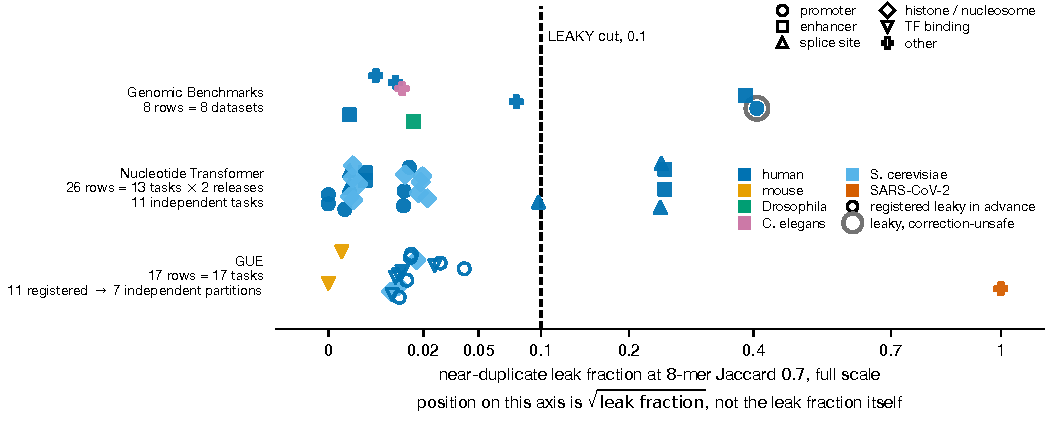
\includegraphics[width=\textwidth]{fig_census}
\caption{Near-duplicate leak fraction across the fifty-one dataset--task censuses reported here, in three benchmark suites. Each point is one censused dataset--task \emph{row}, which is not the same as an independent task, and the panel annotates both conventions: the Nucleotide Transformer contributes $13$ shipped tasks in two releases ($26$ rows) that collapse to $11$ independent tasks, GUE ships $17$ tasks of which the $11$ registered in advance collapse to $7$ independent test partitions, and the text reports independent-task counts throughout. $x$ is the fraction of test sequences whose maximum $8$-mer Jaccard to any training sequence exceeds $0.7$, measured at full scale; position on the axis is the \emph{square root} of that fraction, as the axis label states, so the sub-$0.1$ region, which holds forty-four of the fifty-one, is legible. Marker shape denotes task type ($13$ promoter, $7$ enhancer, $6$ splice site, $13$ histone-mark or nucleosome occupancy, $7$ transcription-factor binding, and five singletons: open chromatin, coding-versus-intergenomic, human-versus-worm, three-class regulatory assignment and nine-way viral variant assignment); colour denotes source organism. The dashed rule at $0.1$ is the LEAKY verdict cut used throughout. Open symbols are the eleven GUE tasks registered in advance as leaky; all eleven fall left of the cut, at $0.009$ to $0.041$. The single grey-haloed point is \textit{human\_nontata\_promoters}, the one dataset certified \emph{leaky-but-correction-unsafe} (Table~1 of the main text). The SARS-CoV-2 point at $1.000$ is \textit{virus\_covid}, where near-identity is a property of the genome rather than a curation defect (\S4). A fourth suite, BEND, is censused in coordinate space only and appears in Fig.~1B of the main text.\label{fig:census}}
\end{figure}



\section{Out-of-suite coordinate census: BEND}\label{sec:s-bend}
Because the screen needs only shipped coordinates it runs outside the suite, at lengths far beyond anything audited here in sequence space. Applied unchanged to the four supervised tasks of BEND \citep{marin2024bend}, whose BED releases carry their own split assignments, it returns $0.000$ at $\ge50\%$ reciprocal overlap on chromatin accessibility ($1{,}410{,}554$ train against $372{,}153$ test intervals), $0.000$ on histone modification ($433{,}861$ against $120{,}567$) and $0.000$ on enhancer annotation in all ten folds---the last at $100{,}096$\,bp per sample (Fig.~1B of the main text). Gene finding, the one task partitioned at $80\%$ identity rather than by chromosome, reproduces the \textit{drosophila\_enhancers\_stark} pattern: $0.183$ of its $597$ test intervals touch a training interval at ${\ge}1$\,bp, yet only $0.002$ reach $\ge50\%$ and none $90\%$. This is the only prospective construction-based call in the paper, and it is near-tautological on the three chromosome-split partitions. Together with the $7/8$ in-suite separation, the screen therefore reads construction defects across four orders of magnitude of interval length without being refitted to the suite it was developed on.

\section{Manipulation replication, all arms}\label{sec:s-manipreps}
\paragraph{Replication: a design, not an anecdote.} With one donor and one recipient the manipulation is $n=1$ per direction, so we repeated break-a-clean on two further clean donors with nothing retuned---the same target duplication share, rate algebra, arms, split seed and evaluation. The manufactured \emph{inflation} replicates on all three. At matched size and balance, \textit{human\_enhancers\_cohn} goes from a clean control (forest drop $-0.003$, CI $[-0.021,0.016]$) to an imposed leak fraction of $0.184$ with a drop of $+0.076$ $[0.059,0.094]$, and \textit{drosophila\_enhancers\_stark} from $-0.000$ $[-0.032,0.033]$ to $0.194$ and $+0.066$ $[0.030,0.101]$; both control intervals include zero and both manipulated intervals exclude it. The manufactured \emph{reordering} replicates on two of the three, and the exception is informative rather than awkward: on \textit{drosophila\_enhancers\_stark} the forest is already rank~4 as shipped, so there is no demotion available for the defect to produce, and it stays rank~4 despite the inflation. Imposing this construction reliably inflates a memorization-prone model; whether that inflation also reorders depends on where the model started.

Separately, the fix-a-leaky direction compared arms of unequal size ($154{,}842$ against $81{,}868$), leaving open whether the merged arm's lower score was the merge or simply less training data. A size-matched control---the unmerged assembly downsampled to the manipulated arm's exact $81{,}868$ rows---still carries leakage ($0.209$) and still inflates the forest ($+0.066$ $[0.055,0.075]$, rank~$2\to4$), so the effect is not an artifact of the size difference (\texttt{results/construction\_manipulation\_replication.csv}).

\section{Robustness arms in full}\label{sec:s-robust}
\paragraph{The block bootstrap.} That the intervals move little is not because the dependence is absent. The splitter assigns whole components to one side, so every near-duplicate relation surviving correction is test-to-test by construction, and the corrected test sets are the more clustered arm: $43.4\%$ of corrected \textit{human\_nontata\_promoters} test sequences lie in a multi-member component against $25.2\%$ as shipped, and $47.7\%$ of \textit{human\_enhancers\_ensembl}'s against $10.1\%$. Those sizes are heavy-tailed, so Kish's $m^{*}$ is $4.45$ and $2.58$ where the mean is $1.55$ and $1.33$, giving design effects of $2.80$ and $2.58$ for the forest where the mean-size convention returns $1.29$ and $1.33$. The inflation is measured directly: on the corrected arm the cluster-bootstrap variance of the forest's accuracy exceeds its sample-bootstrap variance by $3.96\times$ and $2.12\times$ ($3.10\times$ and $1.78\times$ for logistic regression), widening the delta intervals $1.2$--$1.8\times$. The intraclass correlation is high ($0.78$--$0.99$) across the four fits, so the design effect is governed by the block-size distribution rather than by the within-block correlation. The dependence is therefore real, larger than a mean-size design effect suggests, concentrated in the arm the correction creates---and already inside every reported interval, because the block bootstrap resamples those components rather than modelling them. No interval and no verdict changes: the forest's drop still excludes zero on both datasets ($[0.155,0.173]$; $[0.092,0.126]$), and Benjamini--Hochberg over the declared $15$-delta family leaves the same set significant. One source no test-set resampling reaches is the fit, which is held fixed.

\paragraph{Chromosome holdout.} The demotion reproduces on \textit{human\_enhancers\_ensembl}: the forest falls from rank~1 ($0.8596$) to rank~4 ($0.7069$), giving the identical corrected order as the near-duplicate-aware split. On \textit{human\_nontata\_promoters} it does \emph{not}: the forest stays rank~1 ($0.9284\to0.8199$), a third independent signal---with the AUROC/$F_1$ reversal and the novel-only rank correlation---that its demotion is accuracy-only. Two disclosures bound that arm: its test set is $74.33\%$ positive against a $47.20\%$ training prevalence, a $27$-point shift, and it is scored on accuracy, which the imbalance panel below shows understates the correction. The controls agree on the drop magnitude on \textit{human\_enhancers\_ensembl} (corrected $0.707$ against $0.696$); on \textit{human\_nontata\_promoters} they agree to $0.0001$ across test sets $74.3\%$ and $54.4\%$ positive, which is consistent with, but no evidence for, the near-duplicate-aware split proxying the deployment control.

\paragraph{Metric geometry and cluster structure.} The demotion survives canonical (reverse-complement-collapsed) $k$-mer features (forest $1\to4$, drop $0.153$ on \textit{human\_enhancers\_ensembl}; $1\to3$, drop $0.097$ on \textit{human\_nontata\_promoters}), so it is not forward-strand overfitting, and a GC-in-distribution restriction gives \emph{lower} corrected accuracy ($0.787$, $0.631$), not the inflated original, so it is not a GC covariate shift. An MMseqs2 alignment-scored re-clustering reproduces the effect on \textit{human\_enhancers\_ensembl} ($0.164$ against $0.162$) and gives a milder drop on \textit{human\_nontata\_promoters} ($0.108\to0.064$); that arm changes clustering engine and linkage rule together, so the difference is a linkage signature as much as a metric one (Supplementary \S S3). Cluster cohesion explains the asymmetry between the two datasets, and geometrically rather than biologically: \textit{human\_enhancers\_ensembl}'s clusters are $99.6\%$ pairwise at cohesion $0.96$, discrete $2\times$ locus duplication that whole-cluster correction removes cleanly, whereas \textit{human\_nontata\_promoters}'s $420$-member largest component sits at cohesion $0.083$, is $420/420$ \emph{negative} class, and is a single locus tiled by $251$\,bp windows at a median $2$\,bp step---window geometry, not chained paralogy. That geometry has a documented origin rather than an inferred one, though not the one a reader might guess. The negatives are read from a third-party FASTA that already contains $27{,}731$ uniformly $251$\,bp records, and the curators' \texttt{seq2loc} step only recovers their GRCh38 coordinates by exact string match; it does not create the windows and nothing merges them afterwards. The tiling is visible in the notebook's own printed output, whose consecutive chr1 negatives sit at steps of $23$, $8$, $41$ and $32$\,bp---eight rows of a preview, so corroboration of our census rather than a census in itself. Dataset-wide $94.3\%$ of its negatives sit in multi-member components against $0.4\%$ of positives and $2{,}808$ of $2{,}811$ components are class-pure, the same fact \S3.2 reports as $R_{\mathrm{self}}=0.961$ in the negative class; the certification tool therefore returns \emph{leaky-but-correction-unsafe} rather than \emph{leaky} below cohesion $0.5$. A \texttt{dustmasker} check excludes a microsatellite artifact but is silent on interspersed repeats, and on \textit{human\_nontata\_promoters} the leaked stratum is in fact ${\sim}7\times$ AluY-enriched relative to novel (Supplementary \S S3).

\paragraph{Where the multiplicity family is drawn.} Correcting the per-dataset grid and the cross-suite grid as separate families is more permissive than correcting their union, so we ran the union. Pooling all $31$ deltas into one Benjamini--Hochberg family leaves every conclusion in this paper unchanged and adds one flag rather than removing any: \textit{enhancers}$|$LinearSVC crosses at $q=0.049$. Pooling is not the one-sided stress test it looks like---enlarging a family raises the number of tests, which is restrictive, but it also raises the rank of each $p$-value when the incoming tests are more significant than the incumbents, and the per-dataset family contributes several $p$-values below $10^{-5}$. Both effects are real and the analysis has to be run rather than reasoned about (\texttt{results/bh\_pooled.csv}).

\paragraph{Against a published tool.} hashFrag \citep{rafi2026} is the closest runnable comparator: BLAST-based, alignment-scored, and strand-explicit, building its database from both orientations of every training sequence. Run on all eight datasets, it agrees on the two verdicts that matter and disagrees in an instructive way about the rest. Its threshold is the whole story. hashFrag supplies no default and its documentation recommends scoring dinucleotide-shuffled sequences and cutting above that null; done per dataset, that procedure returns thresholds of $21$--$88$ and calls \emph{every} dataset leaky, including all six we call clean. That is the failure our own supplement predicts on independent grounds---real genomic DNA carries repeats and low-complexity tracts that shuffling destroys, so a synthetic null puts the cut far below the scale of real alignment scores---and it is a caution about the recommended procedure rather than about the tool. Sweeping the threshold instead, a window at $220$--$240$ reproduces $7$ of our $8$ verdicts exactly, with per-sequence agreement of $0.837$ on \textit{human\_enhancers\_ensembl} and $0.958$ on \textit{human\_nontata\_promoters} and Cohen's $\kappa$ of $0.636$ and $0.913$ respectively. The separation is in the right direction and is not an artifact of choosing that window: the two leaky datasets require thresholds of $260$ and $380$ before their leak fractions fall under the verdict cut, against $100$--$220$ for the clean ones.

The single persistent disagreement is \textit{drosophila\_enhancers\_stark}, which hashFrag calls leaky at every threshold we swept while we call it clean, and it marks the real boundary of our instrument rather than an error in either tool. Its sequences are long ($2{,}142$\,bp median) and tile the genome, so neighbouring tiles share flanking sequence over hundreds of bases: BLAST scores those alignments highly, while an $8$-mer Jaccard is bounded by the length ratio and stays low. The dataset is clean of near-duplication and is not clean of homology---the same distinction the measured recall of \S4 quantifies, arrived at through a second tool and a different algorithm. Symmetrically, a single absolute alignment score is itself length-dependent: at threshold $220$ hashFrag reads \emph{lower} than we do on \textit{human\_enhancers\_ensembl} ($0.271$ against $0.384$), because that dataset's short sequences cannot reach $220$ at all. Neither instrument is threshold-free, and both should have their cut follow sequence length.

\paragraph{Imbalance, and what ``corrected'' means.} Under induced prevalence imbalance the inflation is revealed by prevalence-aware metrics and masked by accuracy: on \textit{human\_enhancers\_ensembl} at $\pi=0.2$ correction lowers AUPRC $0.622\to0.477$, MCC $0.422\to0.182$ and minority recall $0.258\to0.070$ while accuracy barely moves ($0.844\to0.808$), and on \textit{human\_nontata\_promoters} AUPRC falls $0.949\to0.813$ and MCC $0.785\to0.682$ against accuracy's $0.934\to0.903$---but minority recall is flat there ($0.673\to0.674$), so the recall collapse does not replicate. What generalizes is that AUPRC and MCC fall several times further than accuracy on both datasets, so accuracy at threshold $0.5$ understates the correction; the panel is random-forest-only and its prevalence induced rather than native, leaving the reordering claim untested under imbalance. Across the four robustness arms---block bootstrap, chromosome holdout, metric geometry and induced imbalance---no interval and no verdict changes, and the dependence the block bootstrap measures is real, larger than a mean-size design effect suggests, and already inside every reported interval.

\section{Imbalanced evaluation: full panel}\label{sec:s-imbres}
Table~\ref{tab:imb} gives the prevalence panel at $\pi=0.2$. What generalizes across both datasets
is that AUPRC and MCC fall several times further than accuracy---by $0.145$ and $0.241$ on
\textit{human\_enhancers\_ensembl} against accuracy's $0.036$, and by $0.136$ and $0.103$ on
\textit{human\_nontata\_promoters} against accuracy's $0.030$---so accuracy understates the
correction on both. The minority-recall collapse does \emph{not} generalize: it is specific to
\textit{human\_enhancers\_ensembl} ($0.258\to0.070$) and flat on
\textit{human\_nontata\_promoters} ($0.673\to0.674$), where minority recall ($0.001$) and balanced
accuracy ($0.019$) both move less than accuracy ($0.030$).

\begin{table}[htbp]
\centering
\caption{Prevalence stress test at $\pi=0.2$, random forest, as-shipped $\to$ corrected. The panel
is random-forest-only and the prevalence is induced by downsampling both train and test, not
native, so it does not test the reordering claim under imbalance.}\label{tab:imb}
\footnotesize
\begin{tabular}{@{}lcc@{}}
\toprule
Metric & \textit{h.\ enhancers\_ensembl} & \textit{h.\ nontata\_promoters}\\
\midrule
Accuracy        & $0.844\to0.808$ & $0.934\to0.903$\\
AUPRC           & $0.622\to0.477$ & $0.949\to0.813$\\
MCC             & $0.422\to0.182$ & $0.785\to0.682$\\
Minority recall & $0.258\to0.070$ & $0.673\to0.674$\\
\bottomrule
\end{tabular}
\end{table}

\section{Extended results: controls, grids and the injected multiclass arm}\label{sec:s-tabs}

\begin{figure}[htbp]
\centering
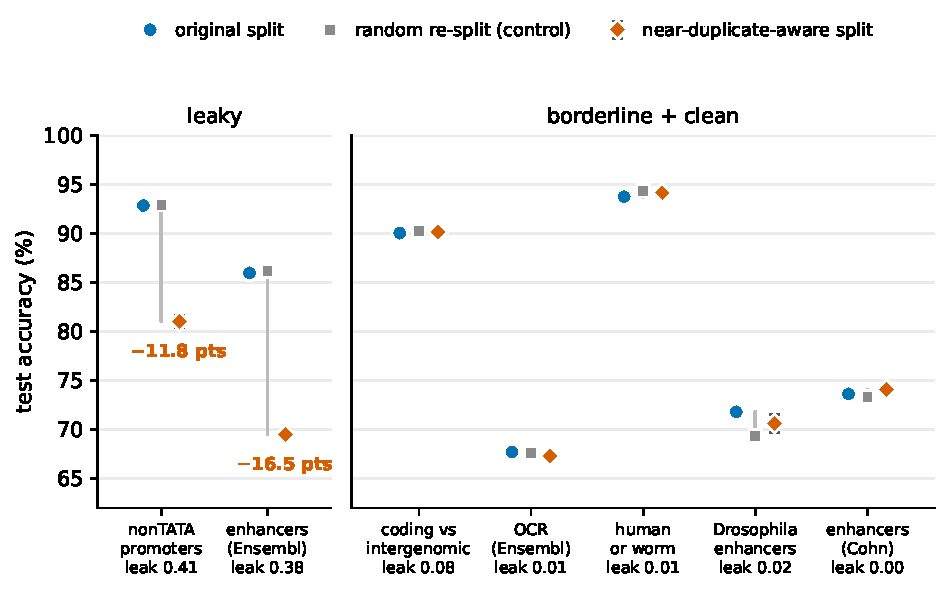
\includegraphics[width=\textwidth]{fig_controls}
\caption{Original split versus random re-split (negative control) versus near-duplicate-aware
re-split, best model per dataset, for all seven binary datasets. On the two leaky datasets (left)
the near-duplicate-aware split costs substantial accuracy while the matched random re-split does
not. On the borderline and clean datasets (right) both deltas are null---the largest,
\textit{drosophila\_enhancers\_stark}, moves $+0.012$ under the near-duplicate-aware split against
$+0.025$ under the random control. That the control sometimes moves a clean dataset further than the
near-duplicate-aware split is the expected behaviour of a null. The best model is the random forest
on the two leaky datasets and logistic regression on the other five, both at $k$=6; ``leak'' is the
near-duplicate test fraction at Jaccard $0.7$; error bars on the corrected points are the standard
deviation over re-split seeds. The random-control deltas are computed on the pre-reconciliation
decision rule and are not directly differenced against the corrected values.}\label{fig:controls}
\end{figure}

\begin{figure}[htbp]
\centering
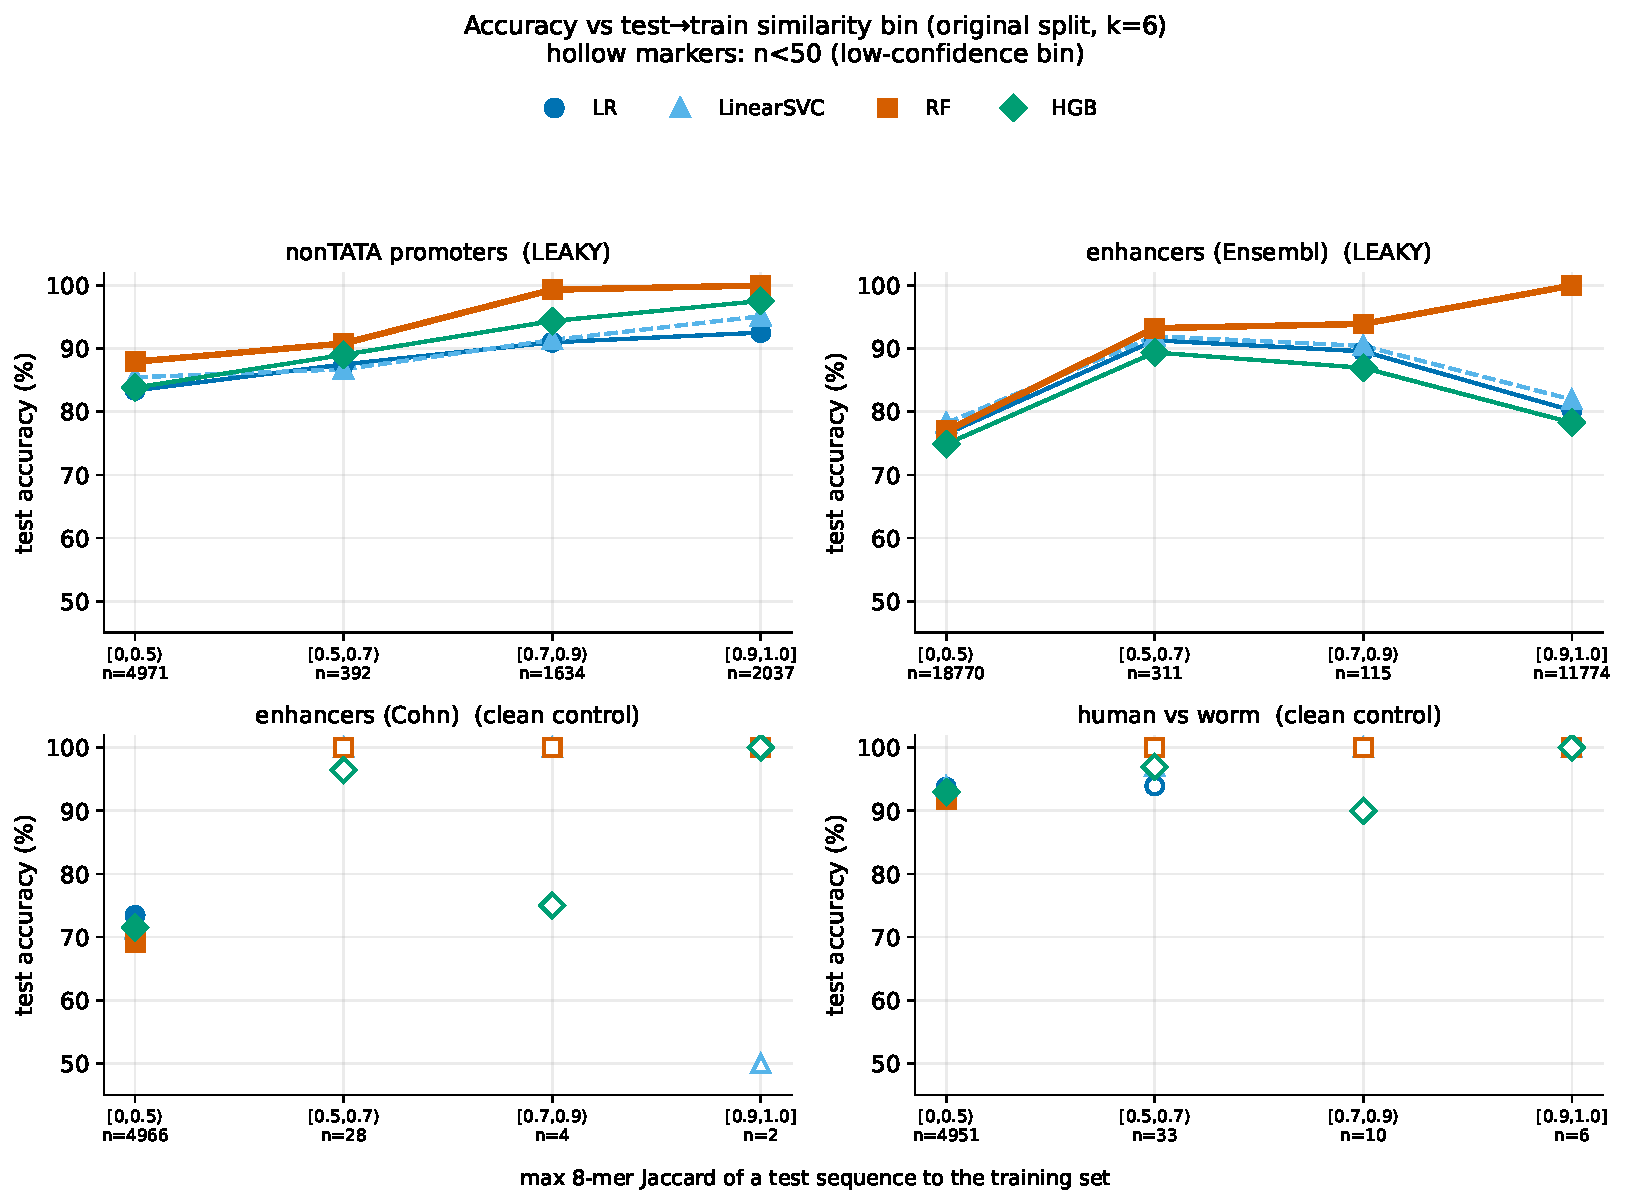
\includegraphics[width=\textwidth]{fig_graded_performance}
\caption{Accuracy as a function of the test-to-train similarity bin (as-shipped split, $k$=6, the
four-model comparison). On leaky datasets the near-default random forest is near-perfect on
high-similarity (near-duplicate) test sequences and falls on dissimilar ones; clean controls have
near-empty high-similarity bins. Hollow markers denote bins with $n<50$.}\label{fig:graded}
\end{figure}

\paragraph{Regularization path (\texttt{results/exp\_regpath.csv}).} Twenty-two rows sweeping
\texttt{min\_samples\_leaf}$\in\{1,5,20,50,100,200,500\}$ and
\texttt{max\_depth}$\in\{\text{None},16,8,4\}$ at full scale on both leaky datasets, reporting per
cell the as-shipped and corrected accuracy, the drop, the graded gap and the model's rank on each
split. The endpoints quoted in the main text are its first and last leaf-size rows. Note the single
$0.0012$ non-monotonicity in the last \textit{human\_nontata\_promoters} leaf-size step, and that
regularization lowers corrected accuracy on that dataset ($0.820\to0.785$) while removing the
inflation, so the two interventions are not interchangeable.

\paragraph{CNN grid (\texttt{results/exp\_deep\_cnn.csv}).} Twenty cells: nine grid cells plus one
unregularized-to-convergence manipulation check per dataset, each with as-shipped accuracy,
corrected accuracy, drop, cluster-bootstrap interval and graded gap. Nineteen of the twenty drop
with intervals excluding zero. The sole exception is the \textit{human\_nontata\_promoters}
dropout-$0.6$, weight-decay-$10^{-4}$ cell, where accuracy rises $0.020$ after correction; we report
that anomaly bare rather than explaining it, since that cell's graded gap of $0.284$ is the largest
of the ten on the dataset and is not consistent with a simple under-fitting account. The
unregularized-to-convergence check memorizes hardest on \textit{human\_enhancers\_ensembl} (graded
gap $+0.222$, drop $+0.076$ $[0.068,0.084]$); on \textit{human\_nontata\_promoters} that same cell's
graded gap is $0.075$, second-lowest of ten, so the ``memorizes hardest'' reading is specific to the
first dataset. Each cell is a single run.

\paragraph{Injected-leakage multiclass arm.} The classical arm
(\texttt{results/exp\_inject3class.csv}) is one run per model per dose; the deep arm
(\texttt{results/exp\_inject3class\_deep.csv}) is three seeds per dose, Table~\ref{tab:injdeep}.
Seed $1$ underfits throughout, with as-shipped accuracy averaging $0.6856$ against $0.7552$ and
$0.7534$ for the other two seeds; it is retained rather than excluded.

\begin{table}[htbp]
\centering
\caption{Injected-leakage multiclass, deep arm, on \textit{human\_ensembl\_regulatory}.
\emph{Drop} is as-shipped minus corrected accuracy, so a negative value means correction
\emph{raised} accuracy. Here $f$ is the fraction of training rows copied into the test set, giving
realised test-set leak fractions $\varphi=0.29$, $0.44$ and $0.62$ at $f=0.1$, $0.2$ and $0.4$. The
random forest on the identical construction drops $+0.0004$, $+0.1177$, $+0.1791$ and
$+0.2581$.}\label{tab:injdeep}
\footnotesize
\begin{tabular}{@{}lrrrr@{}}
\toprule
CNN drop & $f=0.0$ & $f=0.1$ & $f=0.2$ & $f=0.4$\\
\midrule
seed 0 & $-0.0284$ & $-0.0023$ & $-0.0160$ & $+0.0064$\\
seed 1 & $-0.0659$ & $-0.0524$ & $-0.0609$ & $-0.0502$\\
seed 2 & $-0.0216$ & $-0.0000$ & $+0.0023$ & $+0.0172$\\
\midrule
mean   & $-0.0386$ & $-0.0182$ & $-0.0249$ & $-0.0089$\\
sd     & $0.0239$  & $0.0296$  & $0.0325$  & $0.0362$\\
\bottomrule
\end{tabular}
\end{table}

There is no dose-response: every mean is negative, and the seed standard deviation equals or exceeds
any dose effect. This is the outcome ``memorization propensity, not capacity'' predicts, and it is
the arm that scopes the multiclass generalization claim to the classical memorizer.


\section{Exploratory analyses}\label{sec:s-exploratory}
Everything in this section is exploratory. The prevalence-corrected graded gap was defined
after P1 had been scored on its registered raw form, and the curve-shape comparison was not
registered at all; neither can confirm the hypothesis it bears on.

\paragraph{Exploratory: the prevalence-corrected gap.} Everything from here to the end of this subsection is exploratory and is reported as such. P1 was committed against the \emph{raw} graded gap, and the prevalence-corrected form below was defined after that prediction had been scored, so it cannot confirm the hypothesis it was built to rescue---it can only motivate the prospective test we register at the end of this paragraph. Correcting the class-composition confound \emph{strengthens} the mechanism: from balanced accuracy, $1$-nearest-neighbour, the definitional memorizer, has by far the largest gap ($+0.461$), then extremely randomized trees ($+0.370$) and the forest ($+0.319$), with the linear models ($+0.154$, $+0.144$), naive Bayes ($+0.129$) and, lowest, $15$-nearest-neighbour ($+0.016$)---averaging over fifteen neighbours is what stops a nearest-neighbour rule memorizing. The four memorization-prone learners average $+0.292$ against $+0.165$, a separation the raw statistic does not produce. Memorization pays because near-duplicates carry the label: at $\ge0.9$ similarity $99.99\%$ of near-duplicate test sequences share their nearest training neighbour's label on \textit{human\_enhancers\_ensembl} ($n=11{,}774$) and $99.95\%$ on \textit{human\_nontata\_promoters} ($n=2{,}037$); clean datasets have near-empty high-similarity bins (Supplementary Fig.~S2). The correction is equally informative where it removes a signal: on \textit{human\_nontata\_promoters} the corrected gaps do \emph{not} separate the families---memorizers average $+0.122$ against $+0.179$ for the other five, the largest belonging to the MLP---so the mechanism claim is scoped to \textit{human\_enhancers\_ensembl}. We therefore register the corrected gap forward rather than counting it backward: on the next leaky dataset audited, $1$-nearest-neighbour will carry the largest prevalence-corrected graded gap and the four memorization-prone learners will average a larger corrected gap than the remaining five. That prediction is falsifiable on one dataset, and \textit{human\_nontata\_promoters} above is the case in which it would already have failed.

\paragraph{Exploratory: the shape of the curve, against a published one.} That accuracy grades with training-set similarity, and that models rely on memorized associations where it does, is established by \citet{rafi2026} across three modelling regimes; it is not claimed as novel here, and what this suite adds is a matched clean control and an editable construction step. Their curve is non-monotonic---best at both extremes of homology, worse at intermediate similarity---so ours is worth reporting whether or not it agrees. Binning test sequences by maximum similarity to training and reading \emph{balanced} accuracy, so the prevalence confound above cannot manufacture a shape, the two suites disagree in an interpretable way. The memorizing forest is monotone increasing on both leaky datasets ($0.681\to0.818\to0.910\to1.000$ on \textit{human\_enhancers\_ensembl}; $0.788\to0.922\to0.997\to1.000$ on \textit{human\_nontata\_promoters}), which is what a memorization account predicts and what their non-monotonic curve does not show. The models that do \emph{not} memorize are non-monotonic on both, but in opposite directions: on \textit{human\_nontata\_promoters} logistic regression dips at intermediate similarity ($0.824\to0.755\to0.800\to0.963$), the shape they report, while on \textit{human\_enhancers\_ensembl} it peaks there instead ($0.747\to0.955\to0.886\to0.901$). Two things limit this. The intermediate bins are small on \textit{human\_enhancers\_ensembl}---$311$ and $115$ sequences against $18{,}770$ and $11{,}774$ at the extremes---so the peak rests on few observations; and their regimes reach $196$\,kb contexts and functional divergence between homologs, neither of which a $k$-mer model on ${\le}573$\,bp windows can express. We report the difference rather than resolve it (\texttt{results/graded\_shape\_summary.csv}).


\section{An overlap-free protocol for pretrained models}\label{sec:s-fm}
Two routes would settle whether deployed foundation models inherit this inflation, and neither is
performed here. The first uses the stratum HyenaDNA provably never saw: it inherits the Enformer
interval set and designates chromosomes $14$ and X as held-out pretraining test chromosomes, and
both are present in our data, carrying $6.6\%$ of \textit{human\_enhancers\_ensembl}'s test set and
$15.3\%$ of \textit{human\_nontata\_promoters}'s---the latter unevenly by class ($24.6\%$ of test
negatives against $7.5\%$ of positives, which is itself a confound to handle). The second applies
break-a-clean to \textit{drosophila\_enhancers\_stark} and fine-tunes on both arms under both
splits, manufacturing the contamination inside a genome the model has never seen: $6{,}914$
sequences of at most $3{,}237$\,bp and twelve runs of \texttt{hyenadna-small-32k}. Both are stated
so the gap is priced rather than merely disclaimed.

\section{The Nucleotide Transformer splice mechanism}\label{sec:s-splice}
The splice mechanism is not the cross-species homology an earlier account proposed. Of the leaked test sequences, $65.9\%$ (acceptors) and $68.3\%$ (donors) share the same UniProt entry name with their best training partner---same gene, same organism---and at Jaccard $\ge0.9$ that share \emph{rises} to $77.1\%$ and $82.6\%$, where a homology account predicts it should thin; same-species-different-gene pairs number four of $360$ and four of $372$, so it is not paralogy either. The construction draws each gene's decoy negatives from that gene's own exon, intron and false-positive regions, so redundant windows over one gene span the split; label concordance among leaked pairs is correspondingly poor, $0.819$ and $0.792$ against $0.999$ on both Genomic Benchmarks datasets. That account is offered after the fact, not predicted. Same-species-but-different-gene pairs number four of $360$ and four of $372$, so it is not paralogy; the window-type pairing among same-gene pairs (exon-to-exon, false-positive-to-site, intron-to-site) matches the Spliceator/G3PO+ construction, which draws each gene's decoy negatives from that gene's own exon, intron and false-positive regions. Decomposed, label concordance is $0.725$ and $0.701$ among same-gene pairs against $1.000$ and $0.988$ among cross-gene pairs, so memorizing a near-duplicate is wrong roughly a fifth to a quarter of the time on these tasks.

\section{Use of AI and large language models}\label{sec:s-ai}
Generative AI assistants were used for code drafting, for editorial revision of manuscript prose,
and for adversarial review of the manuscript's claims against the released CSV artifacts. They were
not used to generate, select, or interpret any experimental result: every number reported in the
manuscript and in this supplement is produced by a committed script in the released repository and
is re-derived from the corresponding CSV by \texttt{audit/tools/check\_numbers.py}. The author takes
full responsibility for the content of the submission.

\bibliography{references}

\end{document}
